\documentclass[../main.tex]{subfiles}

\begin{document}
    Laser haben gegenüber herkömmlichen Lichtquellen den Vorteil, dass sie räumlich und zeitlich kohärentes Licht produzieren. Insbesondere für Anwendungen, die auf Inteferenzerscheinungen beruhen, wie sie in der Untersuchung von Festkörperstrukturen vorkommen, ist dies nützlich.\\

    Ziel des Versuchs ist deshalb die Konstruktion und Erprobung eines Nd:YAG-Lasers. Dessen wichtigste Komponenten sind:
    \begin{itemize}
        \item \textbf{Aktives Medium.} Im aktiven Medium finden die atomaren Übergänge statt: also Absorption von Photonen und deren spontante und induzierte Emssion. Letztere ist insbesondere verantwortlich für die \textit{kohärente Erzeugung von Laserlicht}. Für diesen Versuch bilden Neodym-Atome das aktive Medium, mit welchen ein YAG-Kristall dotiert wurde. 
        \item \textbf{Pumpe.} Das aktive Medium muss gepumpt werden, damit überhaupt Absorption stattfinden kann. Hier wird optisch mittels einer \textit{Laserdiode} gepumpt. Durch die induzierte Absorption stellt sich eine \textit{Besetzungsinversion} ein, also eine künstliche Population von höheren Zuständen in den Atomen. 
        \item \textbf{Resonator.} Vom aktiven Medium erzeugte Photonen werden im Resonator verstärkt, sodass eine messbare Laserintensität erzeugt werden kann. Hier besetht der Resonator aus zwei Spiegeln, inmitten von welchen das aktive Medium steht. Die Photonen werden zwischen beiden Spiegeln hin- und her reflektiert und sorgen so für vermehrte induzierte Atomen im aktiven Medium. 
    \end{itemize}
    
    Der Nd:YAG-Laser ist ein Vier-Nivau-System, wie \ref{fig:Einleitung:VierNivauSystem} in dargestellt. Das Pumpen erfolgt zwischen dem $\,^4 I_{9/2}$ Niveau, in der Skizze mit (1) bezeichnet, und dem $\,^4 F_{5/2}$ Niveau (4). Die Erzeugung des Laserlichts kommt durch Übergänge von dem $\,^4 F_{3/2}$ Niveau und dem $\,^4 I_{11/2}$ Niveau.

    \begin{figure}[H]
        \centering
        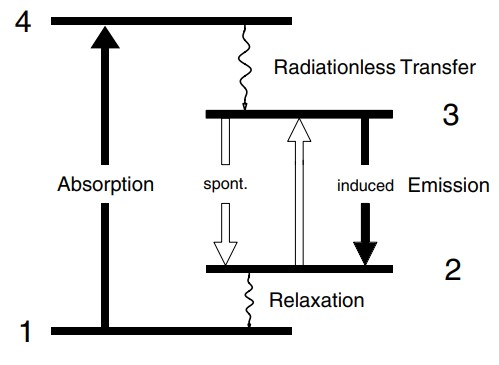
\includegraphics[width=5cm]{Bilddateien/Vier-Niveau-System.jpg}
        \caption{Skizze eines Vier-Niveau-Systems \cite[p.6]{doc:experiment08}}
        \label{fig:Einleitung:VierNivauSystem}
    \end{figure}

\end{document}